\subsection{Kiến trúc Network}
Unity Netcode for GameObjects (NGO) cung cấp nhiều mô hình kiến trúc mạng khác nhau nhằm đáp ứng được nhu cầu của từng loại game multiplayer cụ thể. Mô hình kiến trúc mạng sẽ quyết định cách thức mà dữ liệu được truyền đi giữa các máy, việc máy nào sẽ thực thi logic, cũng như tính bảo mật và hiệu suất của hệ thống. NGO sử dụng 2 kiến trúc mạng chính là Client-Server (dedicated server) và Client-Host. Để lựa chọn được kiến trúc mạng phù hợp theo từng giai đoạn của dự án, sau đây nhóm sẽ phân tích tổng quan về hai kiến trúc mạng trên.
\subsubsection{Mô hình Client-Host}
Trong mô hình Client-Host, có một người chơi sẽ lá Host (vừa là Client, vừa là Server) chạy logic Client như những người chơi khác, đồng thời cũng chạy logic của Server. Các người chơi khác là Client sẽ kết nối tới người chơi Host như một kết nối tới Server.
\begin{figure}[H]
    \centering
    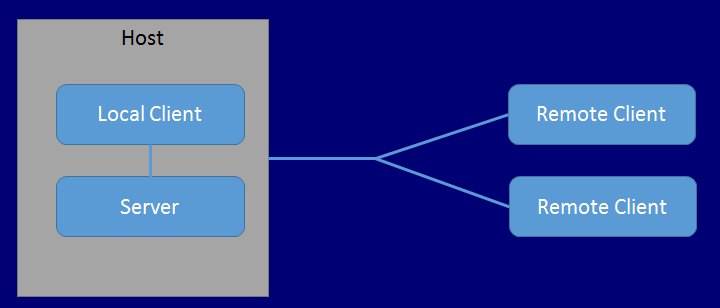
\includegraphics[width=12cm]{4.Cơ sở/images/client-host.png}
    \caption{Mô hình Client-Host}
    \label{fig:ngo-price}
\end{figure}

\begin{itemize}
    \item \textbf{Đặc điẻm chính:}
    \begin{enumerate}[+]
        \item Server ở đây chạy trực tiếp trên máy người chơi (Host).
        \item Không dùng máy chủ riêng.
        \item Máy người chơi Host xử lý toàn bộ logic gameplay và đồng bộ các trạng thái ở máy người chơi client.
    \end{enumerate}
    \item \textbf{Ưu điểm:}
    \begin{enumerate}[+]
        \item Mô hình đơn giản giúp dễ triển khai, phát triển nhanh, phù hợp với game nhỏ.
        \item Không tốn chi phí thuê máy chủ riêng.
    \end{enumerate}
    \item \textbf{Nhược điểm:}
    \begin{enumerate}[+]
        \item Hệ thống phụ thuộc vào cấu hình cũng như mạng của máy Host, máy Host lag thì tất cả người chơi khác đều ảnh hưởng và khi máy Host sập thì game cũng sập.
        \item Tính bảo mật, chống gian lận kém vì người chơi Host quản lý toàn bộ thông tin tất cả người chơi trong phòng và trạng thái gameplay.
    \end{enumerate}
\end{itemize}
\subsubsection{Mô hình Client-Server (Dedicated Server)}
Với mô hình Client-Server, server được chạy trên máy riêng (thường là máy áo), không phải là người chơi. Các người chơi là client sẽ kết nối với server và gửi dữ liệu hoặc gọi lệnh từ server, server sẽ xử lý logic và trả về cho client.
\begin{figure}[!h]
    \centering
    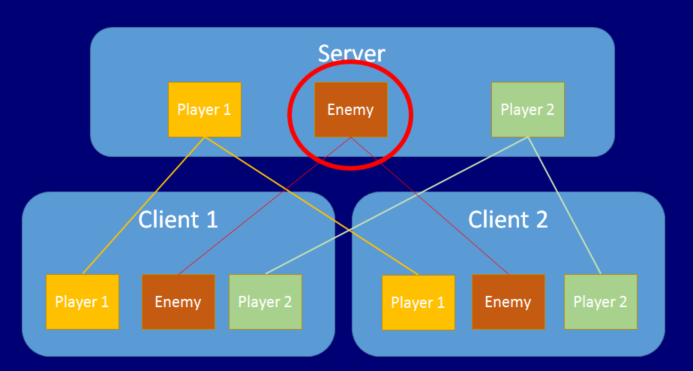
\includegraphics[width=12cm]{4.Cơ sở/images/client-server.png}
    \caption{Mô hình Client-Server (Dedicated Server)}
    \label{fig:client-server}
\end{figure}
\begin{itemize}
    \item \textbf{Đặc điểm chính:}
    \begin{enumerate}[+]
        \item Server là máy chạy độc lập (24/7)
        \item Logic gameplay chỉ được chạy trên server
        \item Client chỉ đóng vai trò hiển thị dữ liệu được server xử lý.
    \end{enumerate}
    \item \textbf{Ưu điểm:} 
    \begin{enumerate}[+]
        \item Tính ổn định cao vì server là máy chạy độc lập, không bị ảnh hưởng bởi người chơi. Người chơi rớt mạng hoặc thoát thì server vẫn chạy.
        \item Tính công bằng, chống gian lận cao do mọi logic và dữ liệu gameplay tập trung ở server, người chơi không có quyền xem dữ liệu người chơi khác cũng như chỉnh sửa dữ liệu gameplay.
        \item Khả năng mở rộng cao khi cần nâng cấp hệ thống (tăng tốc độ truyền, tăng lượng người chơi đồng thời) vì chỉ cần nâng cấp cấu hình máy ảo.
    \end{enumerate}
    \item \textbf{Nhược điểm:} 
    \begin{enumerate}[+]
        \item Tốn chi phí vận hành máy chạy server.
        \item Độ phức tạp cao hơn vì cần có kiến thức về hosting, devops và tối ưu cấu trúc code cho headless server.
    \end{enumerate}
\end{itemize}
\subsubsection{Lý do chọn kiến trúc Client-Host ở giai đoạn phát triển đồ án}
Nhóm quyết định chọn kiến trúc Client-Host cho giai đoạn làm đồ án vì 2 lý do chính là tối ưu tốc độ phát triển dự án và tối ưu về chi phí.
\begin{itemize}
    \item Tối ưu tốc độ phát triển dự án:
    \begin{enumerate}[+]
        \item Kiến trúc Client-Host có thể triển khai dễ dàng trong Unity Editor, không cần triển khai backend, nghiên cứu hosting/devops.
        \item Nhóm phát triền có thể tập trung hơn vào phát triển gameplay, UI của game.
        \item Vì người chơi Host cũng chính là Server nên mỗi lần chơi thử không cần tốn thời gian theo dõi trạng thái server, thuận tiện hơn cho quá trình tìm lỗi.
        \item Giai đoạn phát triển chưa cần quá quan tâm đến độ trễ (không quá ảnh hưởng đến game dạng turn-based) cũng như tính công bằng, bảo mật.
    \end{enumerate}
    \item Tối ưu chi phí: Dự án giai đoạn thử nghiệm ban đầu chưa cần phải thuê dịch vụ máy ảo/hosting nên không tốn chi phí.
\end{itemize}    
\subsubsection{Lý do quyết định chuyển sang kiến trúc Client-Server trong tương lai}
Nhóm dự kiến sẽ chuyển kiến trúc mạng từ Client-Host sang Client-Server trong tương lai, sau khi đã hoàn thiện các logic gameplay cốt lõi và cải tiến UI của game. Mục đính chỉnh của việc này là nhằm tăng chất lượng game về nhiều mặt:
\begin{enumerate}[$\bullet$]
    \item Tính ổn định: Server không còn phụ thuộc vào máy người chơi, điều này giúp cho người chơi có thể ròi phòng bất ký lúc nào (kể cả host) mà không làm gián đoạn game.
    \item Tính công bằng, bảo mật: Chỉ có server mới giữ và xử lý toàn bộ thông tin người chơi và gameplay, người chơi chỉ có quyền xem dữ liệu của bản thân.
    \item Tính mở rộng: Việc xây dựng game trên kiến trúc Client-Server giúp cho nhóm phát triển có thể dễ dàng mở rộng hệ thống game hơn vì khi server không còn là người chơi, việc mở rộng server sẽ trở nên dễ dàng hơn. Các nền tảng phát hành game cũng đòi hỏi điều này đối với các tựa game multiplayer.
\end{enumerate}